Very briefly no zonal flows are found as done in Burin, Tynan etc.
The idea is just to communicating this, without using too much time on this chapter.

If included: Briefly zonal flows comes from Reynold stresses, Diamond and Kim paper shows acceleration of zonal flow comes from radial derivative $\expt{\wt{v}_\theta\wt{v}_r}$ as long as a $\partial_t \grad_\perp^2 \phi$ is present in the system.
%
\begin{figure}[htbp]
    \centering
    \begin{subfigure}[h]{0.45\textwidth}
        \centering
        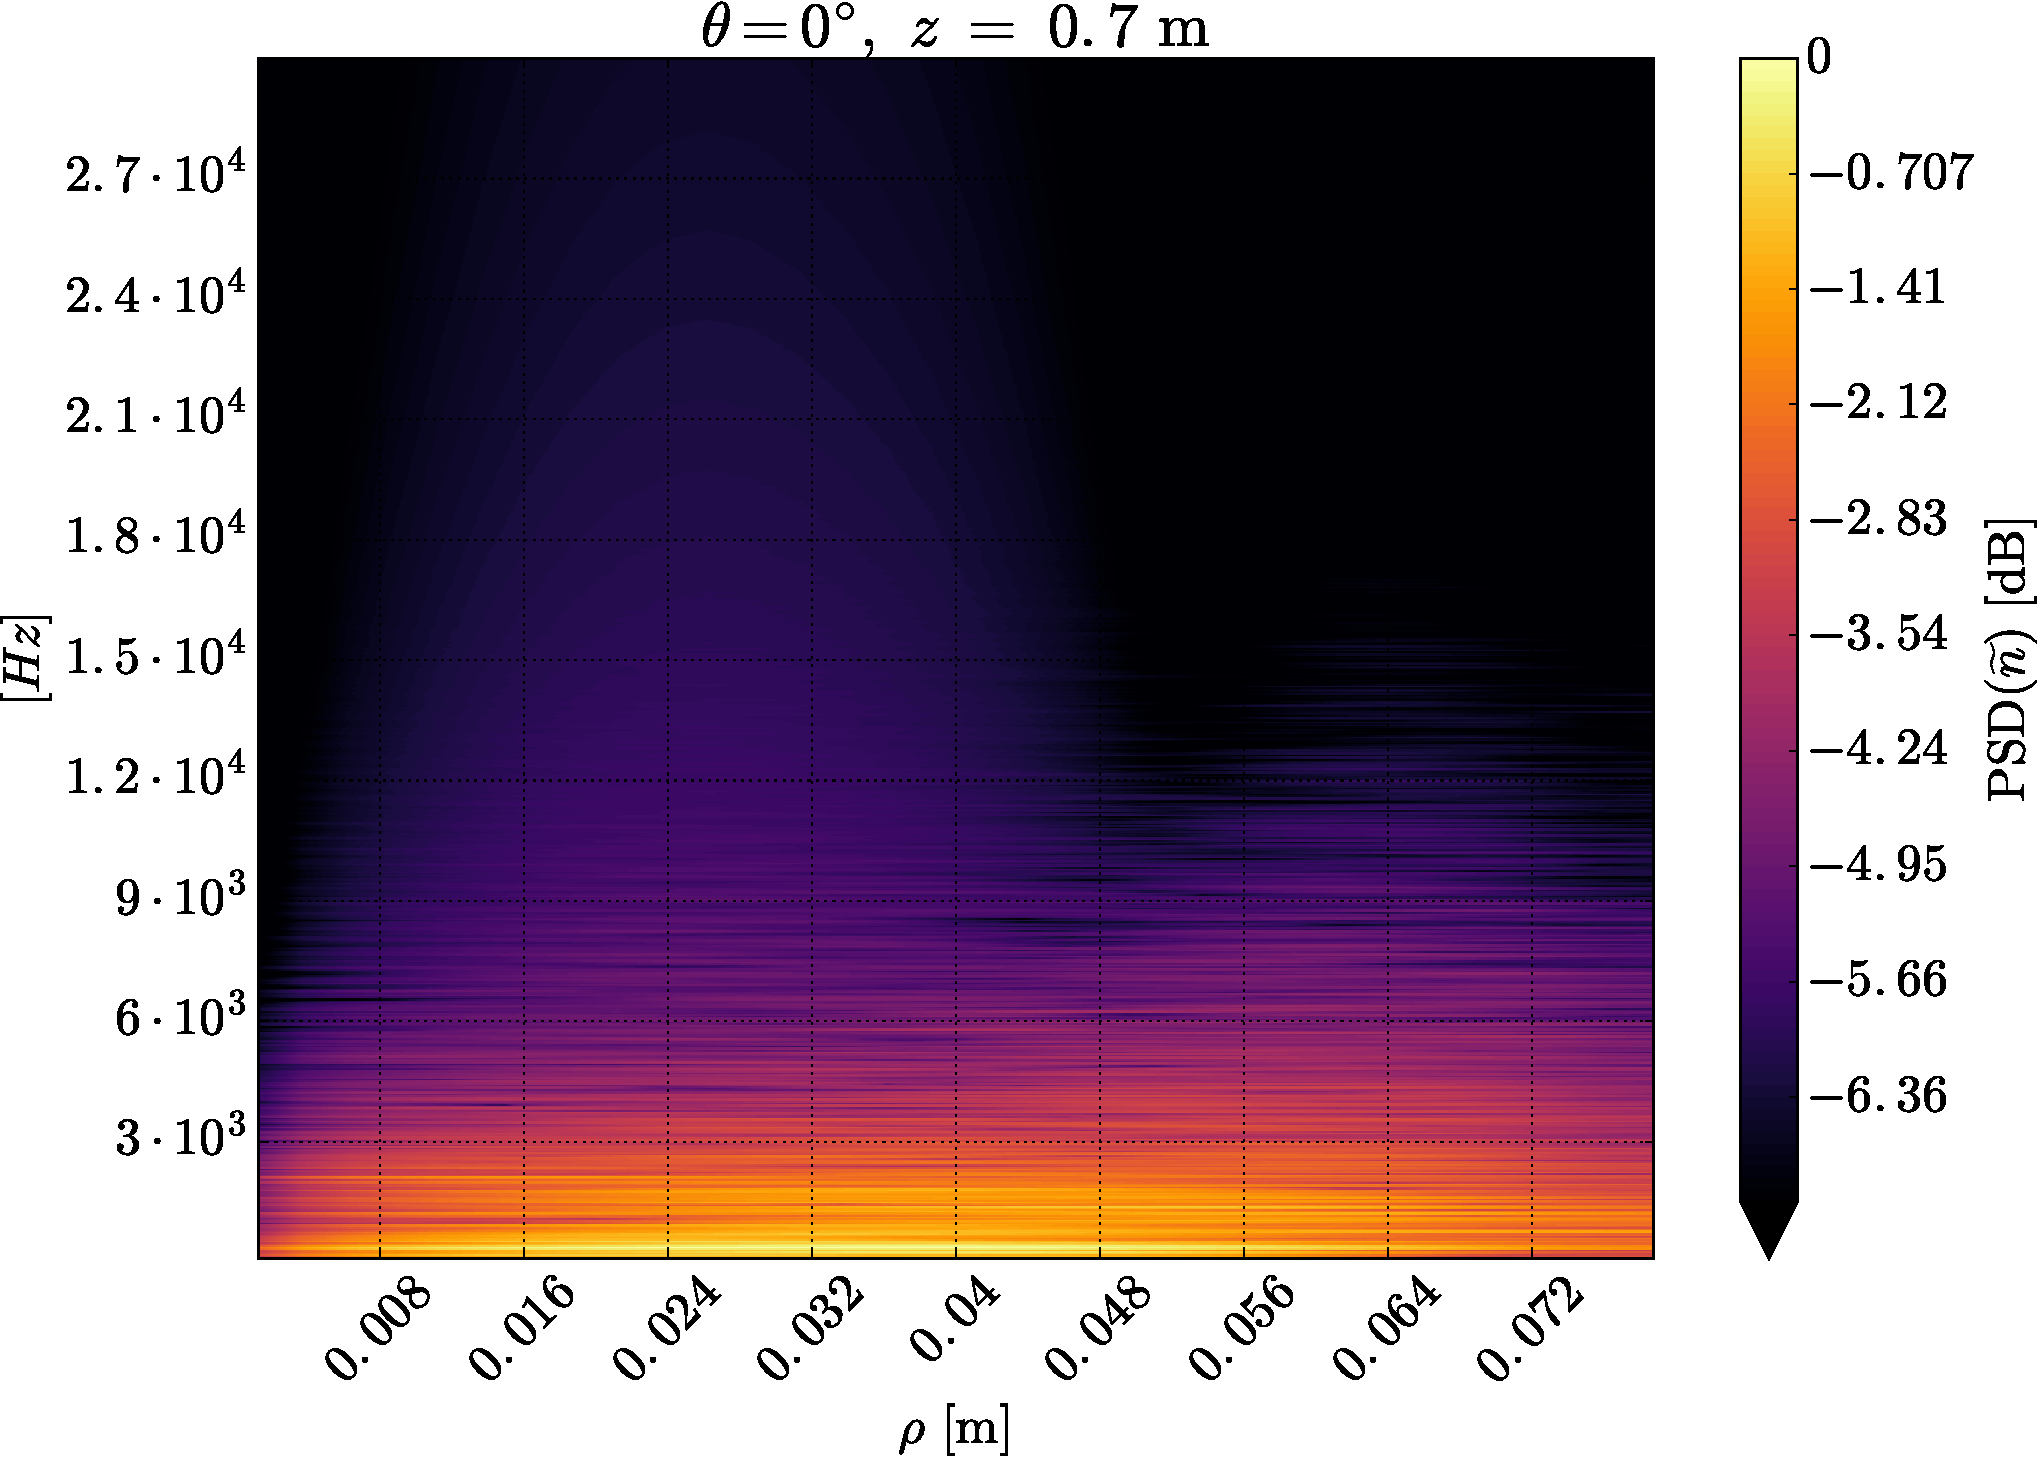
\includegraphics[width=1.0\textwidth]{fig/results/zonal/PSD2D006}
        \label{fig:PSD2D006}
        \caption{$B=0.06\T$}
    \end{subfigure}%
    \hfill
    \begin{subfigure}[h]{0.45\textwidth}
        \centering
        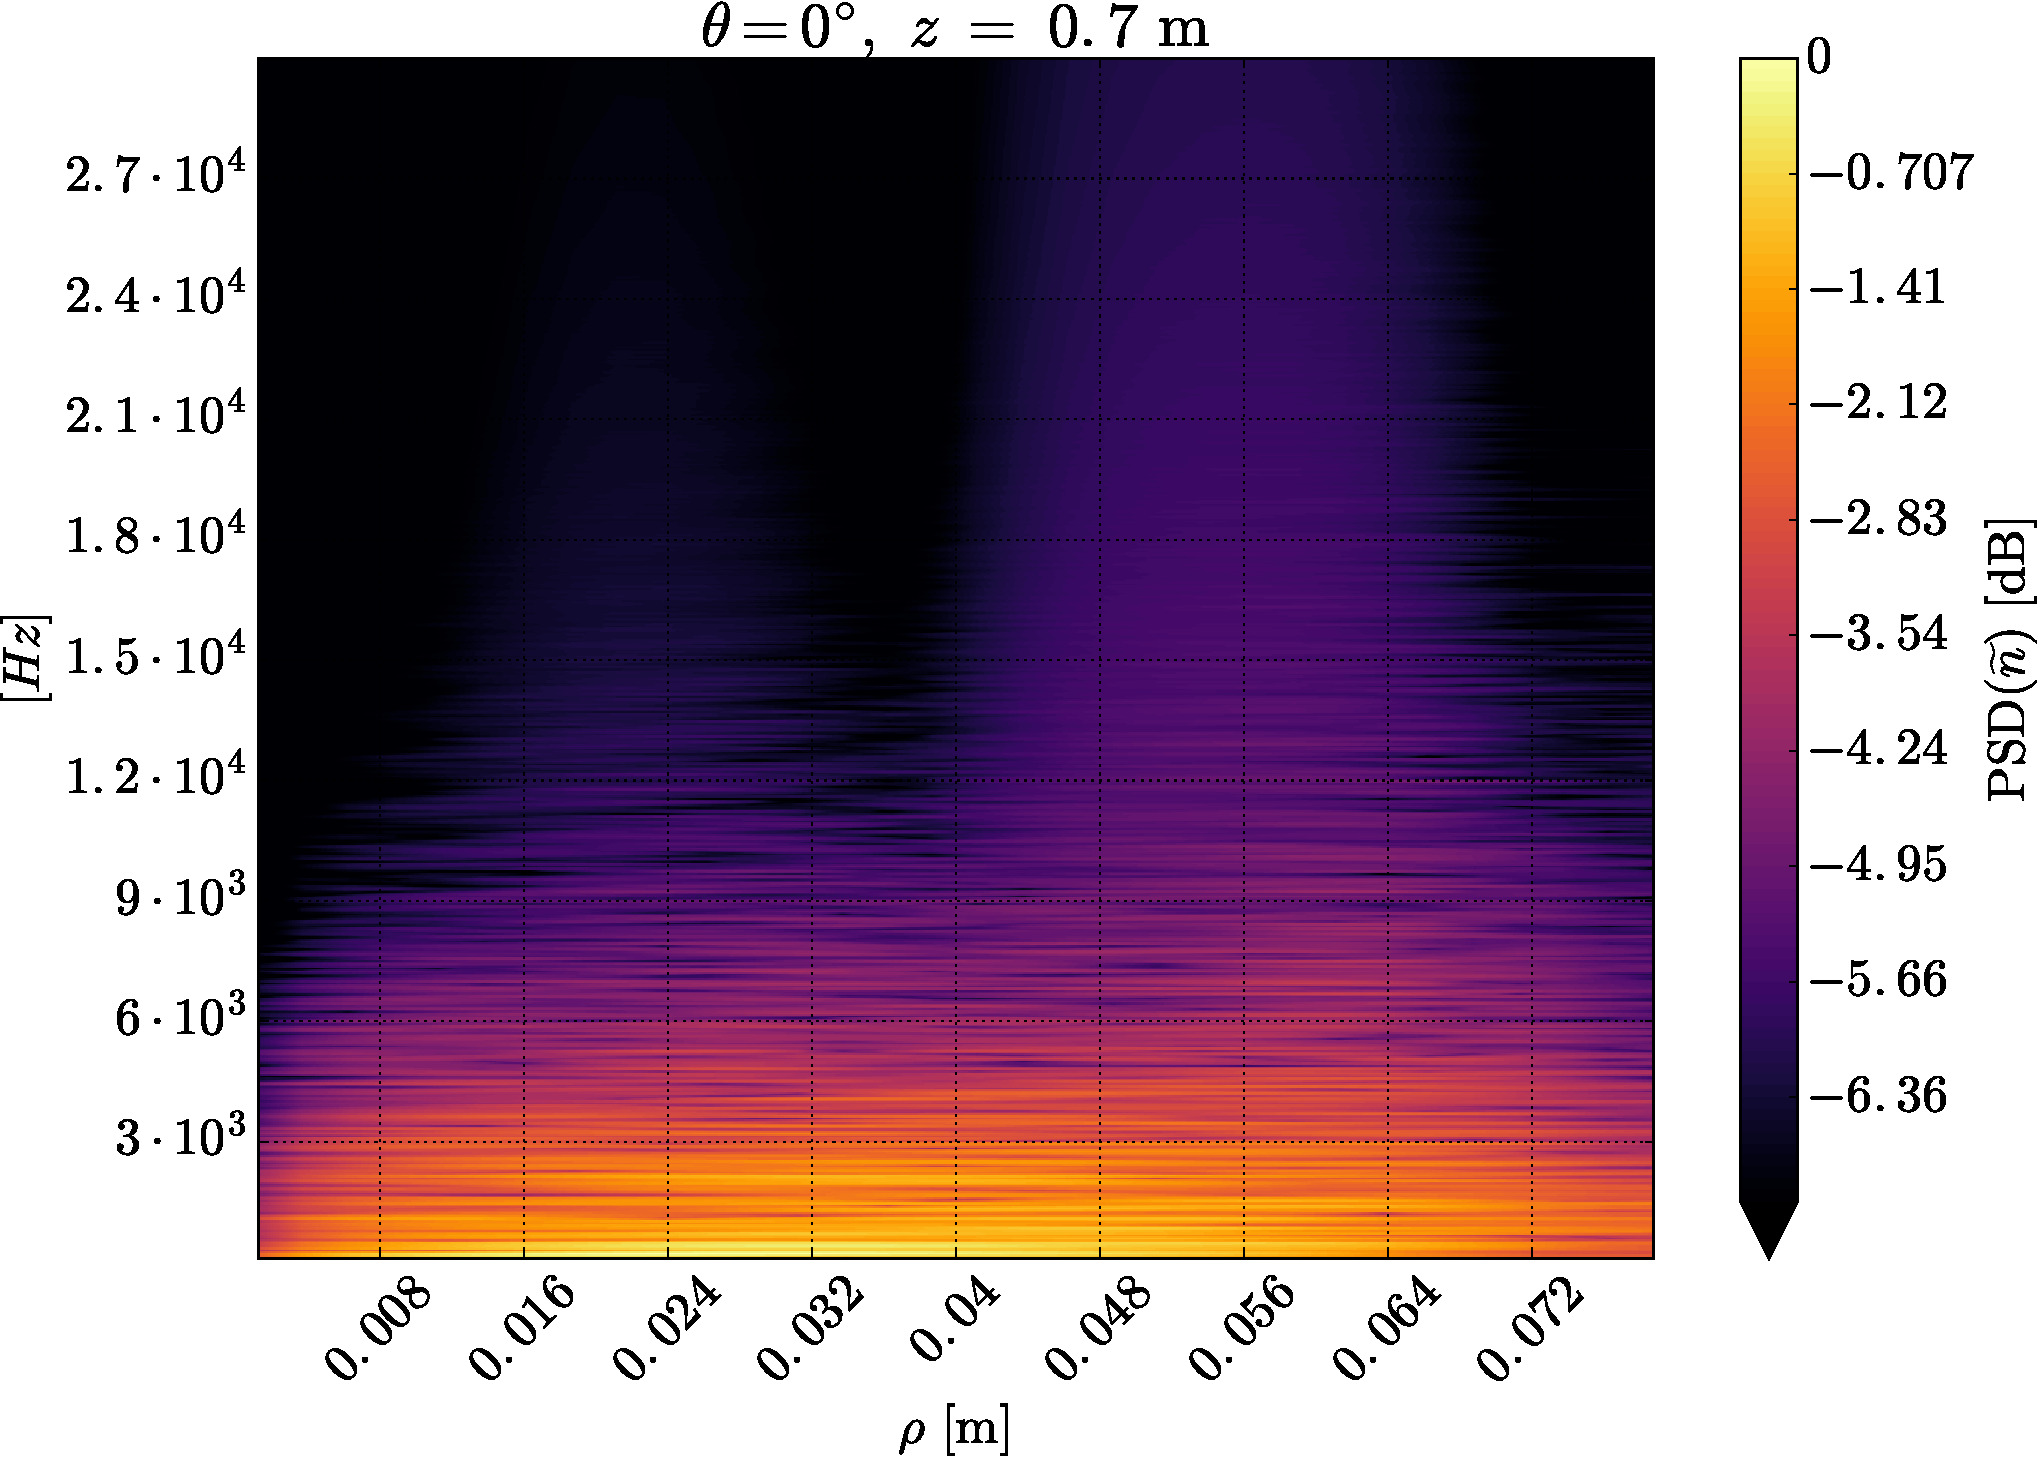
\includegraphics[width=1.0\textwidth]{fig/results/zonal/PSD2D008}
        \label{fig:PSD2D008}
        \caption{$B=0.08\T$}
    \end{subfigure}
    \\
    \begin{subfigure}[h]{0.45\textwidth}
        \centering
        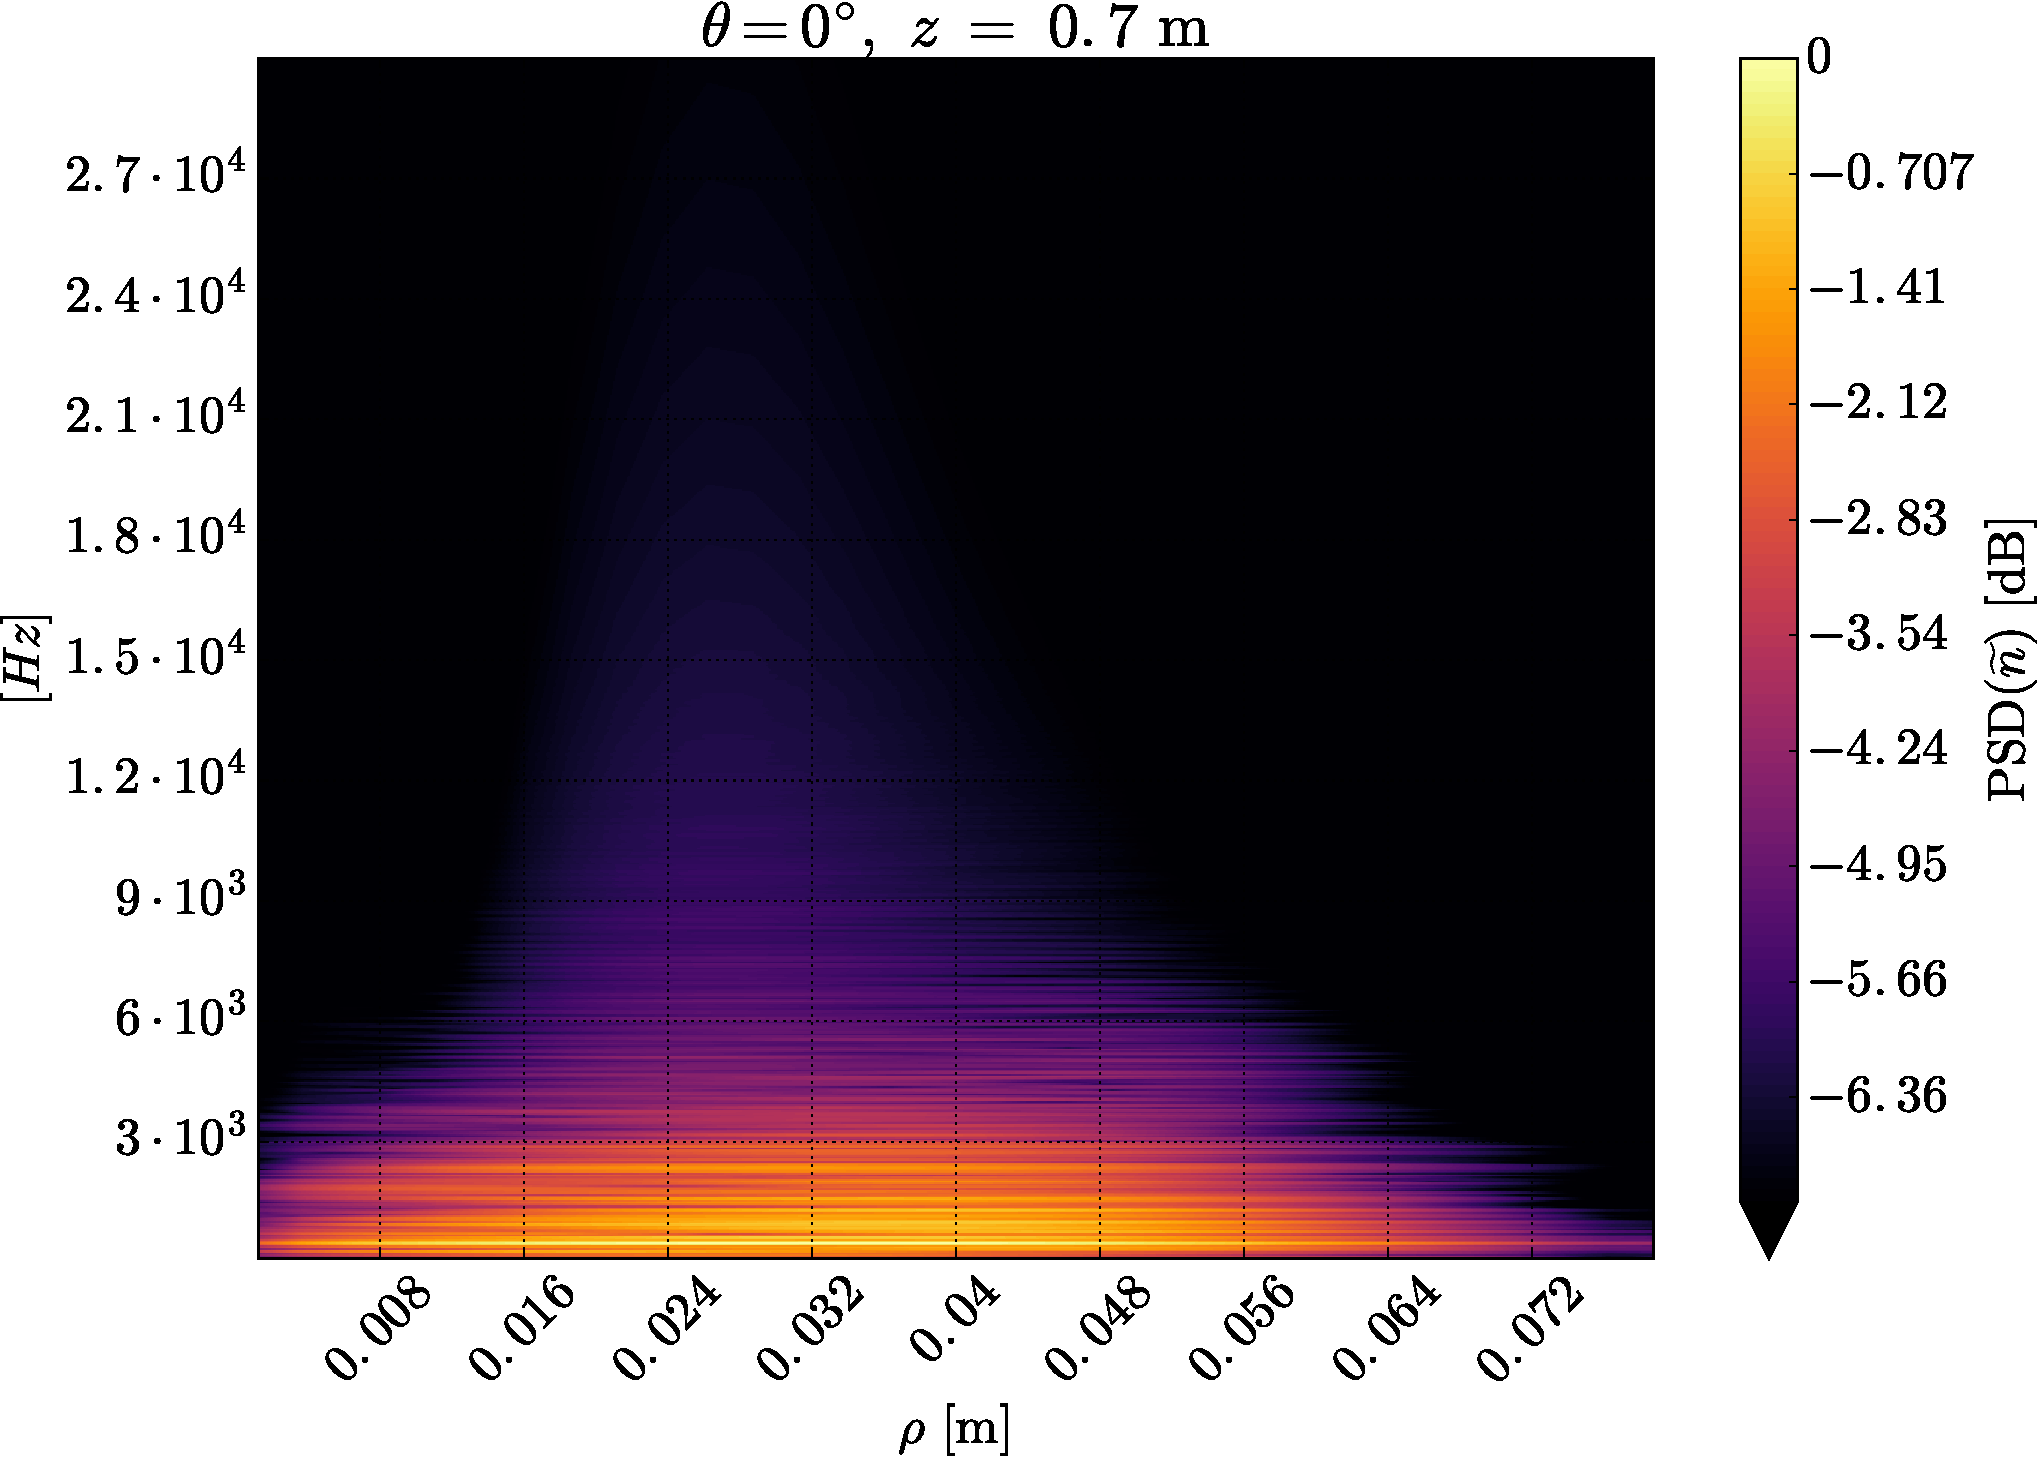
\includegraphics[width=1.0\textwidth]{fig/results/zonal/PSD2D008B}
        \label{fig:PSD2D008B}
        \caption{$B=0.08\T$ using the Boussinesq approximation}
    \end{subfigure}
    \caption{Radial dependency on the power spectral density.}
    \label{fig:PSD2D}
\end{figure}
%
It can be observed in \cref{fig:PSD2D} that the spectra broadens for increasing $B$, and that the main part of the broadening happens outside the maximum of the absolute gradient of $n$.
As stated in ...
the spectra is more narrow when using the Boussinesq approximation.
However, no sustained zonal flow is found from the spectra.
If that was the case, the spectra would be narrowed in the region after the zonal flow as the flow would shear the eddies.
This can also be observed in \cref{fig:zonalFlow0008} which shows a shear only at the very edge of the plasma.
%
\begin{figure}[htb]
    \centering
    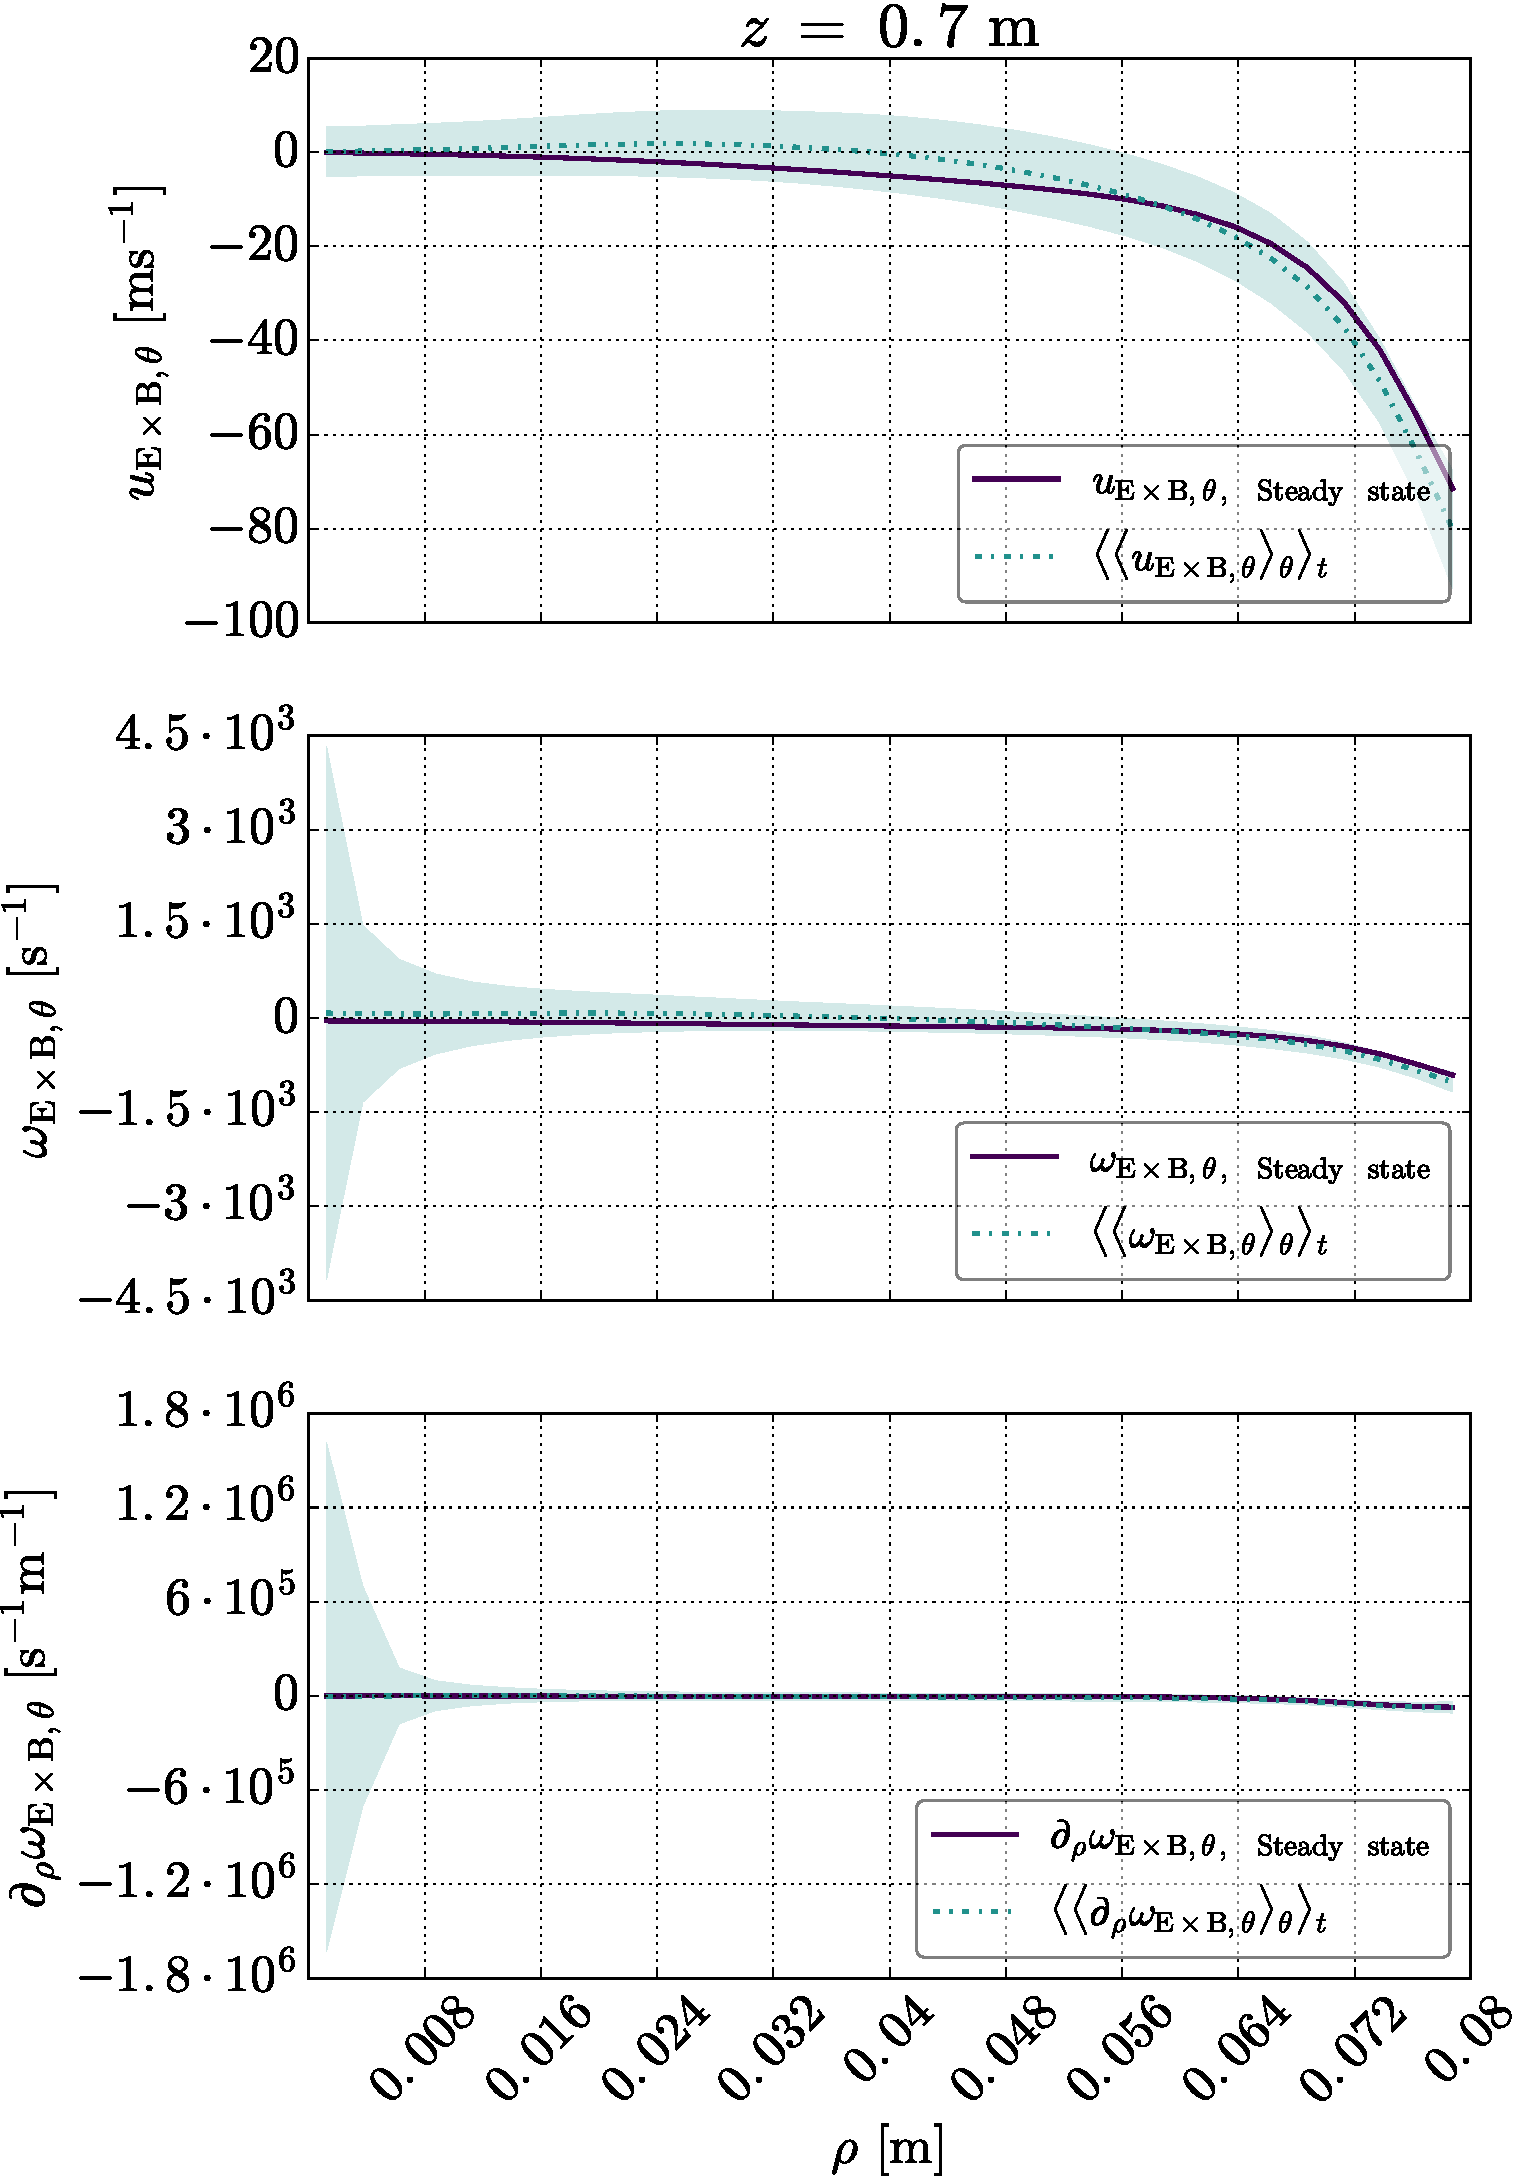
\includegraphics[width=1.0\textwidth]{fig/results/zonal/zonalFlow0008}
    \caption{Poloidal velocity in the system for $B=0.08\T$}
    \label{fig:zonalFlow0008}
\end{figure}
%
